% Source: Code/ML_overlay/ir_rgb_registration/paper/figures/fig_raft_architecture.tex
% RAFT Dual-Encoder Architecture for Cross-Modal IR/RGB Registration
% Experiment 2 — Journal Figure
\documentclass[tikz,border=5pt]{standalone}

\usepackage[T1]{fontenc}
\usepackage{lmodern}
\usepackage{amsmath}

\usetikzlibrary{arrows.meta, positioning, calc, fit, decorations.pathreplacing, shapes.geometric}

% --- Brand Colors ---
\definecolor{Garnet}{HTML}{73000A}
\definecolor{Atlantic}{HTML}{466A9F}
\definecolor{Congaree}{HTML}{1F414D}
\definecolor{Horseshoe}{HTML}{65780B}
\definecolor{Black90}{HTML}{363636}
\definecolor{Black70}{HTML}{5C5C5C}
\definecolor{Black50}{HTML}{A2A2A2}

\begin{document}
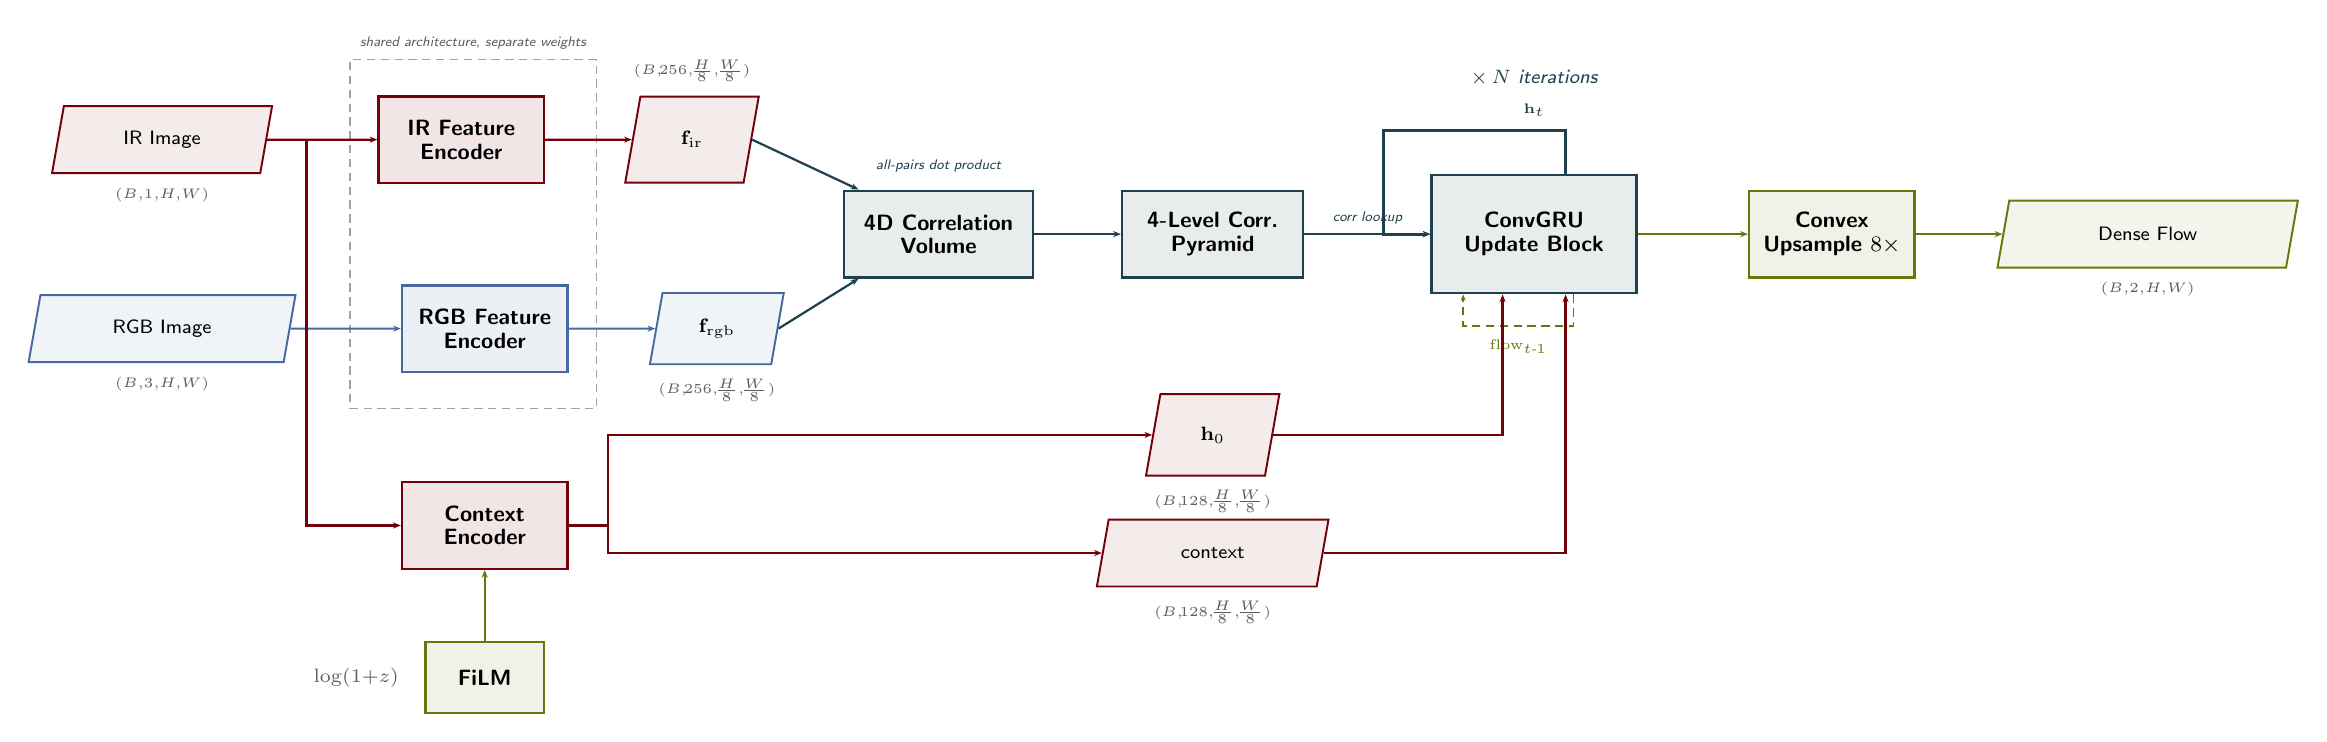
\begin{tikzpicture}[
    >=Stealth,
    font=\sffamily\small,
    procblock/.style={
        draw=#1, fill=#1!10, line width=0.9pt,
        minimum height=11mm, minimum width=21mm,
        inner sep=3pt, align=center,
        font=\sffamily\footnotesize\bfseries,
    },
    tensor/.style={
        draw=#1, fill=#1!8, line width=0.7pt,
        minimum height=8.5mm, minimum width=17mm,
        inner sep=2.5pt, align=center,
        font=\sffamily\scriptsize,
        trapezium, trapezium left angle=80, trapezium right angle=100,
    },
    dimlab/.style={
        font=\sffamily\tiny, text=Black70,
    },
    dataarrow/.style={
        -{Stealth[length=2.8pt,width=2.2pt]},
        line width=0.8pt, color=#1,
    },
    thinarrow/.style={
        -{Stealth[length=2.2pt,width=1.8pt]},
        line width=0.6pt, color=#1,
    },
]

% =====================================================================
% COL 0: INPUTS
% =====================================================================
\node[tensor=Garnet] (ir_in) at (0, 1.2) {IR Image};
\node[dimlab, below=0.5mm of ir_in] {$(B,\!1,\!H,\!W)$};

\node[tensor=Atlantic] (rgb_in) at (0, -1.2) {RGB Image};
\node[dimlab, below=0.5mm of rgb_in] {$(B,\!3,\!H,\!W)$};

% =====================================================================
% COL 1: FEATURE ENCODERS
% =====================================================================
\node[procblock=Garnet, right=14mm of ir_in] (ir_enc) {IR Feature\\[-1pt]Encoder};
\node[procblock=Atlantic, right=14mm of rgb_in] (rgb_enc) {RGB Feature\\[-1pt]Encoder};

% Dashed grouping box
\node[draw=Black50, densely dashed, line width=0.5pt,
      inner xsep=3.5mm, inner ysep=4.5mm,
      fit=(ir_enc)(rgb_enc),
      label={[dimlab, text=Black70, font=\sffamily\tiny\itshape]above:{shared architecture, separate weights}}] {};

% =====================================================================
% COL 2: FEATURE MAPS
% =====================================================================
\node[tensor=Garnet, right=11mm of ir_enc] (fmap_ir) {$\mathbf{f}_{\mathrm{ir}}$};
\node[dimlab, above=0.5mm of fmap_ir] {$\scriptstyle(B,\!256,\!\tfrac{H}{8},\!\tfrac{W}{8})$};

\node[tensor=Atlantic, right=11mm of rgb_enc] (fmap_rgb) {$\mathbf{f}_{\mathrm{rgb}}$};
\node[dimlab, below=0.5mm of fmap_rgb] {$\scriptstyle(B,\!256,\!\tfrac{H}{8},\!\tfrac{W}{8})$};

% =====================================================================
% COL 3: CORRELATION VOLUME
% =====================================================================
\coordinate (corr_mid) at ($(fmap_ir.east)!0.5!(fmap_rgb.east) + (22mm,0)$);
\node[procblock=Congaree, minimum width=24mm] (corr_vol) at (corr_mid) {4D Correlation\\[-1pt]Volume};
\node[dimlab, above=1mm of corr_vol, text=Congaree, font=\sffamily\tiny\itshape] {all-pairs dot product};

% =====================================================================
% COL 4: CORRELATION PYRAMID
% =====================================================================
\node[procblock=Congaree, right=11mm of corr_vol, minimum width=23mm] (corr_pyr) {4-Level Corr.\\[-1pt]Pyramid};

% =====================================================================
% COL 5: ConvGRU UPDATE BLOCK
% =====================================================================
\node[procblock=Congaree, minimum width=26mm, minimum height=15mm,
      right=16mm of corr_pyr]
      (gru) {ConvGRU\\[-1pt]Update Block};

% Recurrent loop arrow over the top
\draw[dataarrow=Congaree, line width=1.0pt]
    ($(gru.north) + (4mm, 0)$) -- ++(0, 5.5mm)
    -| ($(gru.west) + (-6mm, 0)$)
    -- (gru.west);
\node[dimlab, text=Congaree, font=\sffamily\tiny\bfseries, anchor=south]
    at ($(gru.north) + (0, 6mm)$) {$\mathbf{h}_{t}$};
\node[dimlab, text=Congaree, font=\sffamily\scriptsize\itshape, anchor=south]
    at ($(gru.north) + (0, 10mm)$) {$\times\, N$ iterations};

% Flow feedback loop (dashed, underneath GRU)
\draw[thinarrow=Horseshoe, densely dashed]
    ($(gru.south) + (5mm, 0)$) -- ++(0, -4mm)
    -| ($(gru.south) + (-9mm, -4mm)$) -- ($(gru.south) + (-9mm, 0)$);
\node[dimlab, text=Horseshoe, font=\sffamily\tiny\itshape, anchor=north]
    at ($(gru.south) + (-2mm, -4.5mm)$) {$\mathrm{flow}_{t\text{-}1}$};

% =====================================================================
% COL 6: CONVEX UPSAMPLING
% =====================================================================
\node[procblock=Horseshoe, right=14mm of gru, minimum width=21mm] (upsample) {Convex\\[-1pt]Upsample $8{\times}$};

% =====================================================================
% COL 7: OUTPUT
% =====================================================================
\node[tensor=Horseshoe, right=11mm of upsample] (flow_out) {Dense Flow};
\node[dimlab, below=0.5mm of flow_out] {$(B,\!2,\!H,\!W)$};

% =====================================================================
% CONTEXT ENCODER (below RGB pathway)
% =====================================================================
\node[procblock=Garnet, minimum width=21mm]
      (ctx_enc) at ($(rgb_enc) + (0, -2.5)$) {Context\\[-1pt]Encoder};

% FiLM conditioning
\node[procblock=Horseshoe, minimum width=15mm, minimum height=9mm,
      font=\sffamily\footnotesize\bfseries, below=9mm of ctx_enc]
      (film) {FiLM};
\node[dimlab, left=2mm of film, anchor=east, font=\sffamily\scriptsize\itshape] {$\log(1{+}z)$};

% Context encoder outputs -- aligned under corr_pyr for clear separation
\node[tensor=Garnet] (h_state) at ($(corr_pyr) + (0, -2.55)$) {$\mathbf{h}_0$};
\node[dimlab, below=0.5mm of h_state] {$\scriptstyle(B,\!128,\!\tfrac{H}{8},\!\tfrac{W}{8})$};

\node[tensor=Garnet] (ctx_feat) at ($(corr_pyr) + (0, -4.05)$) {context};
\node[dimlab, below=0.5mm of ctx_feat] {$\scriptstyle(B,\!128,\!\tfrac{H}{8},\!\tfrac{W}{8})$};

% =====================================================================
% ARROWS: Main horizontal data flow
% =====================================================================
\draw[dataarrow=Garnet]   (ir_in)  -- (ir_enc);
\draw[dataarrow=Atlantic] (rgb_in) -- (rgb_enc);
\draw[dataarrow=Garnet]   (ir_enc)  -- (fmap_ir);
\draw[dataarrow=Atlantic] (rgb_enc) -- (fmap_rgb);
\draw[dataarrow=Congaree] (fmap_ir.east)  -- ($(corr_vol.north west) + (2mm, 0)$);
\draw[dataarrow=Congaree] (fmap_rgb.east) -- ($(corr_vol.south west) + (2mm, 0)$);
\draw[dataarrow=Congaree] (corr_vol) -- (corr_pyr);
\draw[dataarrow=Congaree] (corr_pyr) -- (gru)
    node[midway, above, dimlab, text=Congaree, font=\sffamily\tiny\itshape] {corr lookup};
\draw[dataarrow=Horseshoe] (gru) -- (upsample);
\draw[dataarrow=Horseshoe] (upsample) -- (flow_out);

% =====================================================================
% ARROWS: Context pathway
% =====================================================================
% IR input forks down to context encoder
\coordinate (ir_fork) at ($(ir_in.east) + (5mm, 0)$);
\draw[dataarrow=Garnet]
    (ir_in.east) -- (ir_fork)
    -- (ir_fork |- ctx_enc.west) -- (ctx_enc.west);

% FiLM --> Context encoder
\draw[dataarrow=Horseshoe] (film.north) -- (ctx_enc.south);

% Context encoder splits to h_0 and context
\coordinate (ctx_split) at ($(ctx_enc.east) + (5mm, 0)$);
\draw[dataarrow=Garnet] (ctx_enc.east) -- (ctx_split) |- (h_state.west);
\draw[dataarrow=Garnet] (ctx_enc.east) -- (ctx_split) |- (ctx_feat.west);

% h_0 --> GRU: route right from h_state then up into GRU south-west
\draw[dataarrow=Garnet]
    (h_state.east) -| ($(gru.south) + (-4mm, 0)$);

% context --> GRU: route right from ctx_feat then up into GRU south
\draw[dataarrow=Garnet]
    (ctx_feat.east) -| ($(gru.south) + (4mm, 0)$);

\end{tikzpicture}
\end{document}
